\chapter{Implementation} \label{ch:implementation}
In this chapter the implementation of the software to control the turntable and the VNA is described based on the design principles laid out in Chapter \ref{ch:design}. The background for the implementation is to fulfill the requirements set out in Chapter \ref{ch:req}. In the project a Windows computer is used to interface to the turntable and VNA, and the software implementation is influenced by this choice. 

The VNA and the turntable are controlled in \textit{Python}. The source code is configured up to have a module for each device and a main control program. In the main control program the concurrency is implemented. The software is programmed with an object-oriented approach. Figure \ref{fig:implementation} shows how variables and  methods are implemented in the VNA and turntable class, and how variables and functions are implemented in the main module.
\begin{figure}[H]
    \centering
    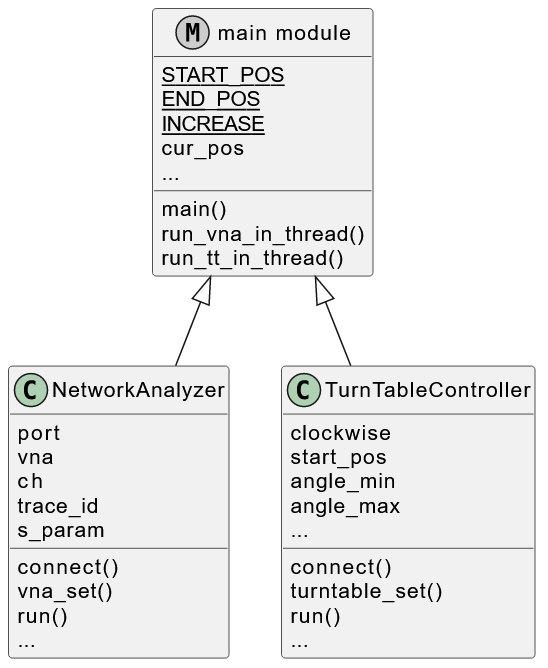
\includegraphics[width=0.5\textwidth]{figures/implementation.png}
    \caption{Diagram of VNA class, turntable class and main module implementation.} \label{fig:implementation}
\end{figure}

\section{Turntable Control}
As previously mentioned in Section \ref{ss:com_interface} the turntable is controlled in \textit{Python} with the \textit{Pywin32} module that gives simple access to the Windows APIs. The turntable comes with a interface documentation document (see \cite{hrt_control_api_manual}) that elaborates on the functions that the turntable will accept. These are implemented in the control program. 

First, a \verb+TurnTableController+ class is defined. The initialisation of the class will call the \verb+__init__+ method that creates the instance variables and tries to connect to the turntable. The connection is checked with a if/elif/else statement. If the connection is not possible, the error handler is set to exit the program. Else, if the connection is established the settings for the turntable will be set. The final \verb+else+ statement is used to catch any other state, which is treated as an error and the program is exited.

The turntable has multiple settings that need to be specified in order to ensure correct operation. These settings are set in the method \verb+turntable_set+ defined in the turntable class in the turntable module, see code in \ref{lst1}. The rpm and the acceleration function are predefined from the manufacturer and can be between 0 and 2 rpm and with four different levels of steepness in acceleration to full speed. Moreover, the turntable can either turn in a bipolar or unipolar direction. The desired unipolar direction is set, however, if this setting can not be made, the \verb+angle_max+ is updated from 360, the unipolar maximum, to 180, the bipolar maximum value. Lastly, the current position \verb+cur_pos+ is read and compared to the start position \verb+start_pos+ in a while loop, and the turntable is instructed to turn to the start position in the opposite direction of its normal turning direction.

\begin{lstlisting} [language=Python, caption=Method to establish settings for turntable and reach start position.]
def __init__(self, instance: str, ttc, clockwise: bool = False, start_pos: float = 0.0, angle_min: float = ANGLE_MIN, angle_max: float = ANGLE_MAX) -> None:
    """ Initalize instance variables, connect and set settings."""
    self.instance = instance
    self.ttc = ttc
    self.clockwise = clockwise
    self.start_pos = start_pos
    self.angle_min = angle_min
    self.angle_max = angle_max
    if self.ttc.Count == 0:
        logger.error("No turntable is connected.")
        exit()
    elif self.connect() == EConnectionState.ecsConnectedOn.value:
        self.turntable_set(rpm=2, func=EAccelerationFunction.afImpulse, start_pos=self.start_pos)
    else:
        logger.error("Unknown error in startup sequence.")
        exit()

def turntable_set(self, rpm: int, func: ´\color{blue}EAccelerationFunction´, start_pos: float) -> None:
    """ Establish basic settings: rpm, acceleration function and start position. """
    cur_pos: int = ´\color{red}round´(self.position)
    try:
        self.tt.Velocity = rpm
        self.tt.AccelerationFunction = func.value
    except ´\color{blue}Exception´ as e:
        logger.´\color{red}error´(f"Unable to set settings for turntable {self.instance}, exiting with error code {e}.")
        ´\color{red}exit´()
    if self.tt.DisplayPolarity == ´\color{blue}EPolarity´.epolBipolar.value:
        try:
            self.tt.DisplayPolarity = ´\color{blue}EPolarity´.epolUnipolar.value
        except ´\color{blue}Exception´:
            self.angle_max = 180.0
            logger.´\color{red}error´(f"Unable to set polarity to unipolar for turntable {self.instance}.")
    while cur_pos != ´\color{red}round´(start_pos):
        logger.´\color{red}info´(f"Current position is {cur_pos} not start position {round(start_pos)}. Moving {self.instance} to start position.")
        if self.clockwise:
            self.´\color{red}go\_to\_CCW´(start_pos)
        else:
            self.´\color{red}go\_to\_CW´(start_pos)
        cur_pos = round(self.position)
    logger.´\color{red}info´(f"Settings are velocity: {round(self.tt.Velocity)}, function: {EAccelerationFunction(self.tt.AccelerationFunction)}.")
    logger.´\color{red}info´(f"Current position for {self.instance} is {cur_pos}.")
\end{lstlisting} \label{lst1}

The \verb+run+ method, see code \ref{lst2}, of the turntable takes the value of the increment \verb+inc+ as input argument and accesses the current position \verb+cur_pos+ and the value of the turning direction \verb+clockwise+ to determine and turn either in a clockwise or counter-clockwise direction. Finally the position is checked against the maximum and minimum angle values which are defined in the beginning of the module to be \verb+ANGLE_MIN = 0.0+ and \verb+ANGLE_MAX = 360.0+.

The \verb+step_CW+ method is equal to the \verb+step_CCW+ method except for the turning direction. First, the size of the step is set before the step is made, according to the definition in the turntable documentation. For the \verb+go_to_CW+ method, the interface method to be called is \verb+GoToCW+ which accepts the position in degrees as a floating point number as input. Both methods include the option to force the program to execute no other tasks while the turntable is turning which is done by setting the \verb+wait+ flag which will call the \verb+wait_while_driving+ method. This method calls \verb+time.sleep()+ which effectively utilises the active processor fully. The \verb+wait_while_driving+ method also includes a wait time check that will break the wait while loop after the user defined timeout and allow the code to continue executing. 

\begin{lstlisting}[language=Python, caption=Methods for turning the turntable to the wanted position.]
def run(self, inc: float) -> None:
    """ Run the turntable. Changes the current position with [inc] degrees. """
    cur_pos: float = self.position
    if self.clockwise:
        self.´\color{red}step\_CW´(inc)
    else:
        self.´\color{red}step\_CCW´(inc)
    if (self.angle_min > cur_pos > self.angle_max):
            logger.´\color{red}error´(f"Current position is illegal. Resetting: {self.instance}")
            self.´\color{red}reset´(self.instance, self.clockwise)

def step_CW(self, degrees, wait: bool = False) -> None:
    """ Step [degrees] in clockwise direction. """
    self.tt.StepSize = float(degrees)
    self.tt.StepCW()
    if wait:
        self.´\color{red}wait\_while\_driving´()

def go_to_CW(self, degrees: float, wait: bool = False) -> None:
    """ Go to [degrees] while moving in clockwise direction. """
    self.tt.GotoCW(float(degrees))
    if wait:
        self.´\color{red}wait\_while\_driving´()

def wait_while_driving(self) -> None:
    """ Ensures that the program waits for the turntable to reach position before execution further code. """
    seconds_waited = 0.0
    while self.tt.IsMoving:
        ´\color{blue}time´.´\color{red}sleep´(0.5)
        seconds_waited += 0.5
        if seconds_waited > 120:
            logger.´\color{red}warning´('Timeout while waiting for stop.')
            break
\end{lstlisting} \label{lst2}

The \verb+reset+ method, see code \ref{lst3}, used in the \verb+run+ method for position check will first call the \verb+stop+ method. This method will force stop the turntable by calling \verb+MoveAbort()+. The \verb+reset+ method then rotates to the start position \verb+start_pos+ based on the setting of the clockwise boolean variable.

\begin{lstlisting}[language=Python, caption=Method for resetting the turntable to start position.]
def stop(self) -> None:
    """ Stop turning. """
    if self.tt.IsMoving:
        self.tt.MoveAbort()
        logger.´\color{red}warning´(f"Turntable was moving while connection was stopped for {self.instance}.")
    logger.´\color{red}info´(f"Turntable {self.instance} is stopped.")

def reset(self) -> None:
    """ Reset Turntable to start position. """
    self.´\color{red}stop´()
    if self.clockwise:
        self.´\color{red}go\_to\_CCW´(self.start_pos)
    else:
        self.´\color{red}go\_to\_CW´(self.start_pos)
\end{lstlisting} \label{lst3}

The turntable class includes a single attribute, which is the position of the turntable. The position is established as an attribute by using the \verb+@property+ decorator on the method returning the position variable. Setting the position as an attribute without a \verb+setter+ decorator ensures that the position variable becomes read-only. 

\section{VNA Control}
The automation of the measurements with the VNA are made with the \textit{Rohde \& Schwarz} instrument library, that provides an easy interface instead of implementing the SCPI commands. Firstly, the connection with the VNA must be established. The IP address of the VNA has been manually set in the settings on the VNA and the assigned port has been extracted from the computer system. 

The VNA control is implemented as a class object. In the \verb+__init__+ method of the class, see code \ref{lst4}, the connection is established to the VNA over TCP. Further, relevant settings are provided as class variables. This is for example the frequency on which the measurements must be made. This is provided as a floating point number when the VNA class is instantiated. The number of measurements, also called channel points, is also set in the \verb+__init__+ method to 1, since only one measurement needs to be made at one frequency. If the measurements should've been made over a frequency range, the \verb+start_frequency_Hz+ and \verb+stop_frequency_Hz+ could be modified accordingly and the number of measurements to be made in the range can be set with the \verb+points+ variable.

The \verb+connect+ method, see code \ref{lst4}, implements an exception handler in case the \verb+open_tcp+ method returns an error and exits the program, because it is not recommended to execute further without this connection. If the connection is successfully established a single channel with the identifier \verb+ch=1+ is created. 

The specific S-parameter to be measured is also set when the class is instantiated. The value is used in the \verb+vna_set+ method that establishes the trace settings, such as which S-parameter to measure and the format of the measurements, which is magnitude in \SI{}{\decibel}.

\begin{lstlisting}[language=Python, caption=Method for initialisation of VNA settings including creating VNA trace.]
def __init__(self, trace_id: str, s_param: str, freq: float, ip_address = '172.0.0.1', port: int = 5025, channel = 1) -> None:
    """ Initalize instance variables and connect.
    Instrument Type: ZVB8 with 2 Ports
    Part Number: 1145.1010k08
    Serial Number: 100113
    Device ID: 1145.1010K08-100113-DD
    IEC Bus Address: 20
    IP Adresses: IP Address 172.0.0.1 (Localhost) Subnet Mask: 255.0.0.0 """
    self.port: int = port
    out: tuple = self.´\color{red}connect´(ip_address, port, channel)
    self.vna: ´\color{blue}Vna´ = out[0]
    self.ch: ´\color{blue}Channel´ = out[1]
    self.trace_id = trace_id
    self.s_param = s_param
    self.ch.start_frequency_Hz = freq, 'GHz'
    self.ch.stop_frequency_Hz = freq, 'GHz'
    self.ch.points = 1

def connect(self, ip_address: str, port: int, ch: int) -> tuple:
    """ Try to connect to VNA with TCP. """
    try:
        sock = ´\color{blue}Vna´()
        sock.´\color{red}open\_tcp´(ip_address, port)
    except ´\color{blue}Exception´ as e:
        logger.´\color{red}error´(f'Cannot connect to VNA because {e}.')
        ´\color{red}exit´()
    else:
        logger.´\color{red}info´(f'Connection established to VNA. Creating channel {ch}.')
        channel = sock.´\color{red}channel´(ch)
        return sock, channel

def vna_set(self) -> None:
    """ Establish trace for VNA. """
    self.vna.create_trace(self.trace_id, 1, self.s_param)
    self.vna.trace(self.trace_id).format = TraceFormat.magnitude_dB
\end{lstlisting} \label{lst4}

The \verb+run+ method, see code \ref{lst5}, returns the data measured formatted as a tuple with frequency at index 0 and power at index 1. The \verb+run+ method calls the \verb+trace+ method from the \verb+Vna+ class from the \textit{Rohde \& Schwarz} instrument library to retrieve the trace ID and calls the \verb+measure_formatted_data+ method on the trace variable. 

\begin{lstlisting}[language=Python, caption=Method for getting measurements from VNA.]
def run(self) -> tuple:
    """Measure S-Parameters for [trace_id]."""
    x, y = self.vna.´\color{red}trace´(self.trace_id).´\color{red}measure\_formatted\_data´()
    return x, y
\end{lstlisting} \label{lst5} 

The VNA can be completely reset by calling the \verb+preset+ method from the \textit{Rohde \& Schwarz} instrument library, however, this will also remove the calibration of the VNA that is performed to normalize the transmission line. The calibration data can be saved as a file and reopened for continuous use of the same calibration data. The calibration must therefore be performed manually before the execution of the setup, otherwise the data can be faulty.

\section{Main Control Flow}
The start and end positions and the angle increase are initialised as constants, see code \ref{lst6}. The current position \verb+cur_pos+ must be read both by the VNA thread and the turntable thread, and must be set by the turntable, therefore this variable is defined globally together with a lock \verb+lock_cur_pos+, so that only one thread will access the variable at a time. Likewise with the variable for maximum position \verb+max_pos+ which also has its own event handler \verb+max_pos_event_handler+, so that the turntable thread will wait for the VNA thread to find the maximum position before reading the variable and turning to that position.
\begin{lstlisting}[language=Python, caption=Global constants and variables.]
START_POS = 10.0
END_POS = 150.0
INCREASE = 20.0

lock_cur_pos = ´\color{blue}Lock´()
cur_pos: int = None

max_pos_event_handler = ´\color{blue}Event´()
lock_max_pos = ´\color{blue}Lock´()
max_pos: int = None
\end{lstlisting} \label{lst6}

The turntable is interfaced with the windows API made available with the \textit{Pywin32} module. The code in line 2-3 in \ref{lst7} in the \verb+run_tt_in_thread+ function is the initialisation of this interface. Then, the global variables are accessed via \textit{Python}'s \verb+global+ keyword. The current position is read from the \verb+turntable.position+ property defined in the \textit{turntable} module. The while loop turns the turntable from the \verb+START_POS+ to the \verb+END_POS+ in increments of \verb+INCREASE+. In the while loop, the turntable sets its own event handler \verb+turntable_event_handler+ to \verb+true+ to indicate to the VNA thread that it can now run, and then the turntable thread waits for the VNA thread. Hereafter the turntable turns and updates the current position \verb+cur_pos+. Once the end position \verb+END_POS+ is reached, the while loop is exited and this is indicated to the VNA thread with the \verb+end+ event handler. Lastly, the turntable thread turns to the maximum position \verb+max_pos+ when the VNA thread has indicated, that this variable has been set. 

\begin{lstlisting}[language=Python, caption=Thread function for running VNA.]
def run_tt_in_thread(ttc: ´\color{blue}CDispatch´, turntable_event_handler: ´\color{blue}Event´, vna_event_handler: ´\color{blue}Event´, end: ´\color{blue}Event´, ttc_id) -> None:
    ´\color{red}CoInitialize´()
    ttc = ´\color{red}Dispatch´(´\color{red}CoGetInterfaceAndReleaseStream´(ttc_id, IID_IDispatch))
    turntable = ´\color{blue}TurnTableController´(instance="hrt i (64980128)", ttc=ttc, clockwise=True, start_pos=START_POS)
    
    global cur_pos
    global max_pos
    count: int = 1

    with lock_cur_pos:
        cur_pos = ´\color{red}round´(turntable.position)

    while START_POS <= cur_pos < END_POS:
        turntable_event_handler.´\color{red}set´()
        turntable_event_handler.´\color{red}clear´()
        vna_event_handler.´\color{red}wait´()
        turntable.´\color{red}run´(INCREASE)
        with lock_cur_pos:
            cur_pos = ´\color{red}round´(turntable.position) 
            ´\color{blue}logging´.´\color{red}info´(f"Current position for {turntable.instance} is {cur_pos}.")
        count += 1
    turntable_event_handler.´\color{red}set´()
    turntable_event_handler.´\color{red}clear´()
    end.´\color{red}set´()

    max_pos_event_handler.´\color{red}wait´()
    with lock_max_pos:
        if turntable.clockwise:
            turntable.go_to_CW(max_pos)
        else:
            turntable.go_to_CCW(max_pos)

    ´\color{blue}logging´.´\color{red}info´(f'Turntable thread is closed. {count} positions measured.')
\end{lstlisting} \label{lst7}

The VNA thread \verb+run_vna_in_thread+, see code \ref{lst8}, first accesses the global variables \verb+cur_pos+ and \verb+max_pos+. Then two lists for measurement position \verb+data_pos+ and measured power \verb+data_pow+ are defined. The while loop for the VNA runs as long as the turntable thread has not set the \verb+end+ event handler to true, indicating that turning has finished. The while loop begins with waiting for the turntable to indicate it has finished turning with the \verb+turntable_event_handler+. The power measurement is made with the execution of the code in line 10 in the VNA thread. The two lists containing the measurement data are updated by first calling the current position lock \verb+lock_cur_pos+ before appending to the lists. When the turntable thread has indicated that turning is finished, the VNA thread immediately calculates the maximum position and updates the global \verb+max_pos+ variable.

\begin{lstlisting}[language=Python, caption=Thread function for running VNA.]
def run_vna_in_thread(vna: ´\color{blue}NetworkAnalyzer´, turntable_event_handler: ´\color{blue}Event´, vna_event_handler: ´\color{blue}Event´, end: ´\color{blue}Event´) -> None:
    global cur_pos 
    global max_pos
    data_pos: list = []
    data_pow: list = []
    count: int = 0 

    while not end.´\color{red}is\_set´(): # run only when end == false
        turntable_event_handler.´\color{red}wait´() 
        _, pow = vna.´\color{red}run´()
        vna_event_handler.´\color{red}set´() 
        vna_event_handler.´\color{red}clear´()
        ´\color{blue}logging´.´\color{red}info´(f'Power measurement is {pow}.')
        with lock_cur_pos: 
            data_pos.´\color{red}append´(cur_pos)
            data_pow.´\color{red}append´(pow)
        count += 1

    max_gain: float = ´\color{red}max´(data_pow)
    with lock_max_pos:
        max_pos = data_pos[data_pow.´\color{red}index´(max_gain)]
    ´\color{blue}logging´.´\color{red}info´(f'Max gain measured is {max_gain} at position {max_pos}.')
    max_pos_event_handler.set() 

    ´\color{blue}logging´.´\color{red}info´(f'VNA thread is closed. {count} measurements made.')
\end{lstlisting} \label{lst8}

The \verb+main+ function, see code \ref{lst9}, has to create the setup for controlling the turntable with the Windows API in a thread, the VNA instance and trace settings, the two threads, event handlers, start the threads and ensure that both threads close correctly when finished by using the \verb+join()+ function on each thread. 
\begin{lstlisting}[language=Python, caption=Main function.]
def main():
    ´\color{blue}logging´.´\color{red}basicConfig´(filename=f'./tests/test-{time.strftime("%Y%m%d-%H%M")}-log.txt', filemode='a', format="%(asctime)s:%(name)s: %(message)s", level=logging.INFO, datefmt="%Y-%m-%d %H:%M:%S")
    
    ´\color{red}CoInitialize´()
    ttc = ´\color{red}Dispatch´("TurnTableControlLib.TurnTableControl")
    ttc_id = ´\color{red}CoMarshalInterThreadInterfaceInStream´(IID_IDispatch, ttc)

    vna = ´\color{blue}NetworkAnalyzer´(trace_id='trc1', s_param='s21', freq=5.65)
    vna.´\color{red}vna\_set´()
    ´\color{blue}logging´.´\color{red}info´(f'VNA with trace id {vna.trace_id} is created. Measuring {vna.s_param}.')
    ´\color{blue}logging´.´\color{red}info´(f'Settings are: {vna.get_settings()}')

    turntable_event_handler = ´\color{blue}Event´()
    vna_event_handler_handler = ´\color{blue}Event´()
    end = ´\color{blue}Event´()

    turntable_thread = ´\color{blue}Thread´(target=´\color{red}run\_tt\_in\_thread´, kwargs={'ttc_id': ttc_id, 'ttc': ttc, 'turntable_event_handler': turntable_event_handler, 'vna_event_handler': vna_event_handler_handler, 'end': end})
    turntable_event_handler.clear()

    vna_thread = ´\color{blue}Thread´(target=´\color{red}run\_vna\_in\_thread´, kwargs={'vna': vna, 'turntable_event_handler': turntable_event_handler, 'vna_event_handler': vna_event_handler_handler, 'end': end})
    
    turntable_thread.´\color{red}start´()
    vna_thread.´\color{red}start´()

    turntable_thread.´\color{red}join´()
    vna_thread.´\color{red}join´()
\end{lstlisting} \label{lst9}
Calling the \verb+main+ function ensures that the entire setup, meaning the turning of the turntable and the measuring of magnitude of the received signal by the VNA, runs automatically before saving the data logs to a text file.